\chapter{EMS Calling Points}\label{ems-calling-points}

This section provides an overview of EnergyPlus's program flow and describes the various places where you can use the EMS to initiate calls for custom controlling. The input object EnergyManagementSystem:ProgramCallingManager requires the user describe the timing for when the Erl programs are run. These \emph{EMS Calling Points} correspond to places inside the EnergyPlus program where and when the EMS can be called to do something. The EMS offers a wide range of calling points. This section attempts to explain what you need to know about the EnergyPlus program flow so you can better understand which calling point to use for a particular application. Because the EMS needs to interact with the rest of the EnergyPlus computer program, you need a fairly high level of understanding of the inner workings of EnergyPlus. Finding the right point to insert your Erl override is a challenge. This is a complicated computer program. Using an interpreted language to override its calculations is no simple thing and should not be taken lightly.

The best calling point will depend on the type of actuator being controlled and the intent of the override activity. Unfortunately, there is no easy way to explain the inner workings of a model as large as EnergyPlus, so this section includes only a brief overview. We attempt to provide useful recommendations for the types of control that are best suited for particular calling points. But for the full details you will need to refer to the EnergyPlus source code, which you can obtain with a developer license.

This section starts with a series of three figures and then discusses them and the 14 calling points. Figure~\ref{fig:overall-program-flow-and-ems-calling-points} shows the overall flow of an EnergyPlus model with some EMS calling points. Figure~\ref{fig:timestep-sequence-with-ems-calling-points} shows the sequence for a single timestep with the remaining EMS calling points. Figure~\ref{fig:system-timestep-sequence-with-ems-calling} is similar but shows the calling points for shortened system timesteps. These diagram the flow of procedures during a run from top to bottom.

\begin{figure}[hbtp] % fig 1
\centering
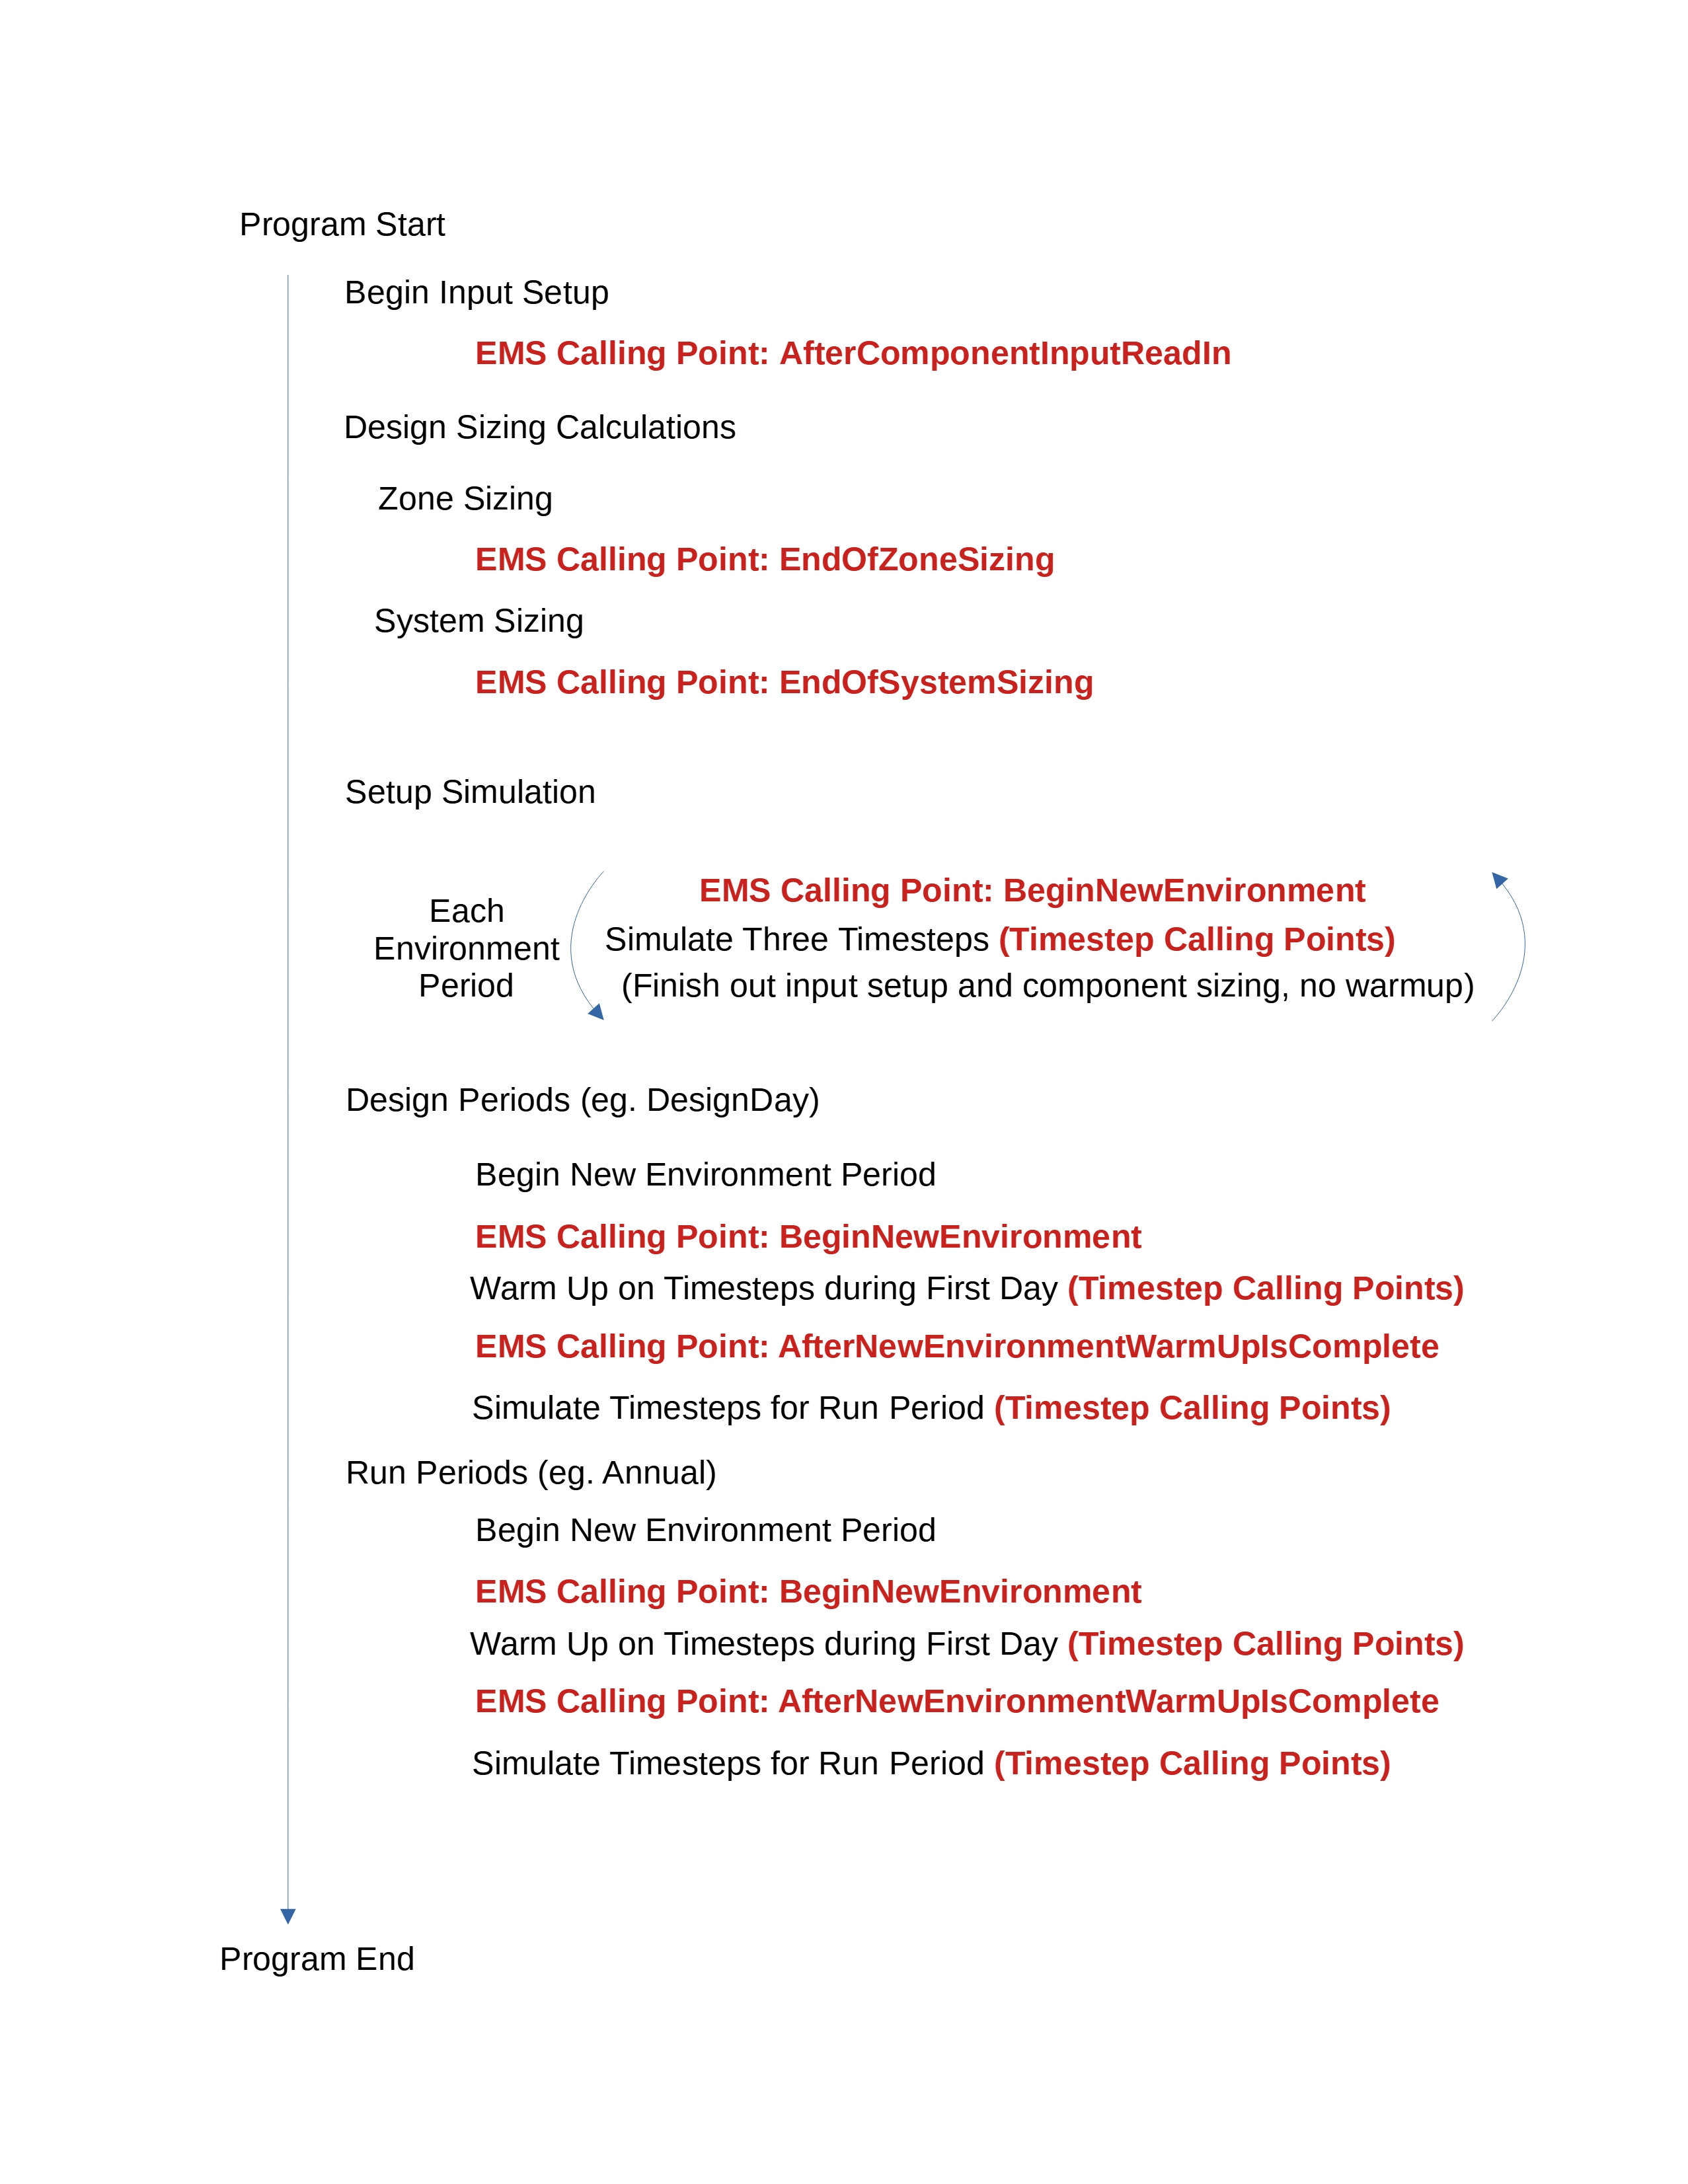
\includegraphics[width=0.9\textwidth, height=0.9\textheight, keepaspectratio=true]{media/image003.jpg}
\caption{Overall Program Flow and EMS Calling Points \protect \label{fig:overall-program-flow-and-ems-calling-points}}
\end{figure}

\begin{figure}[hbtp] % fig 2
\centering
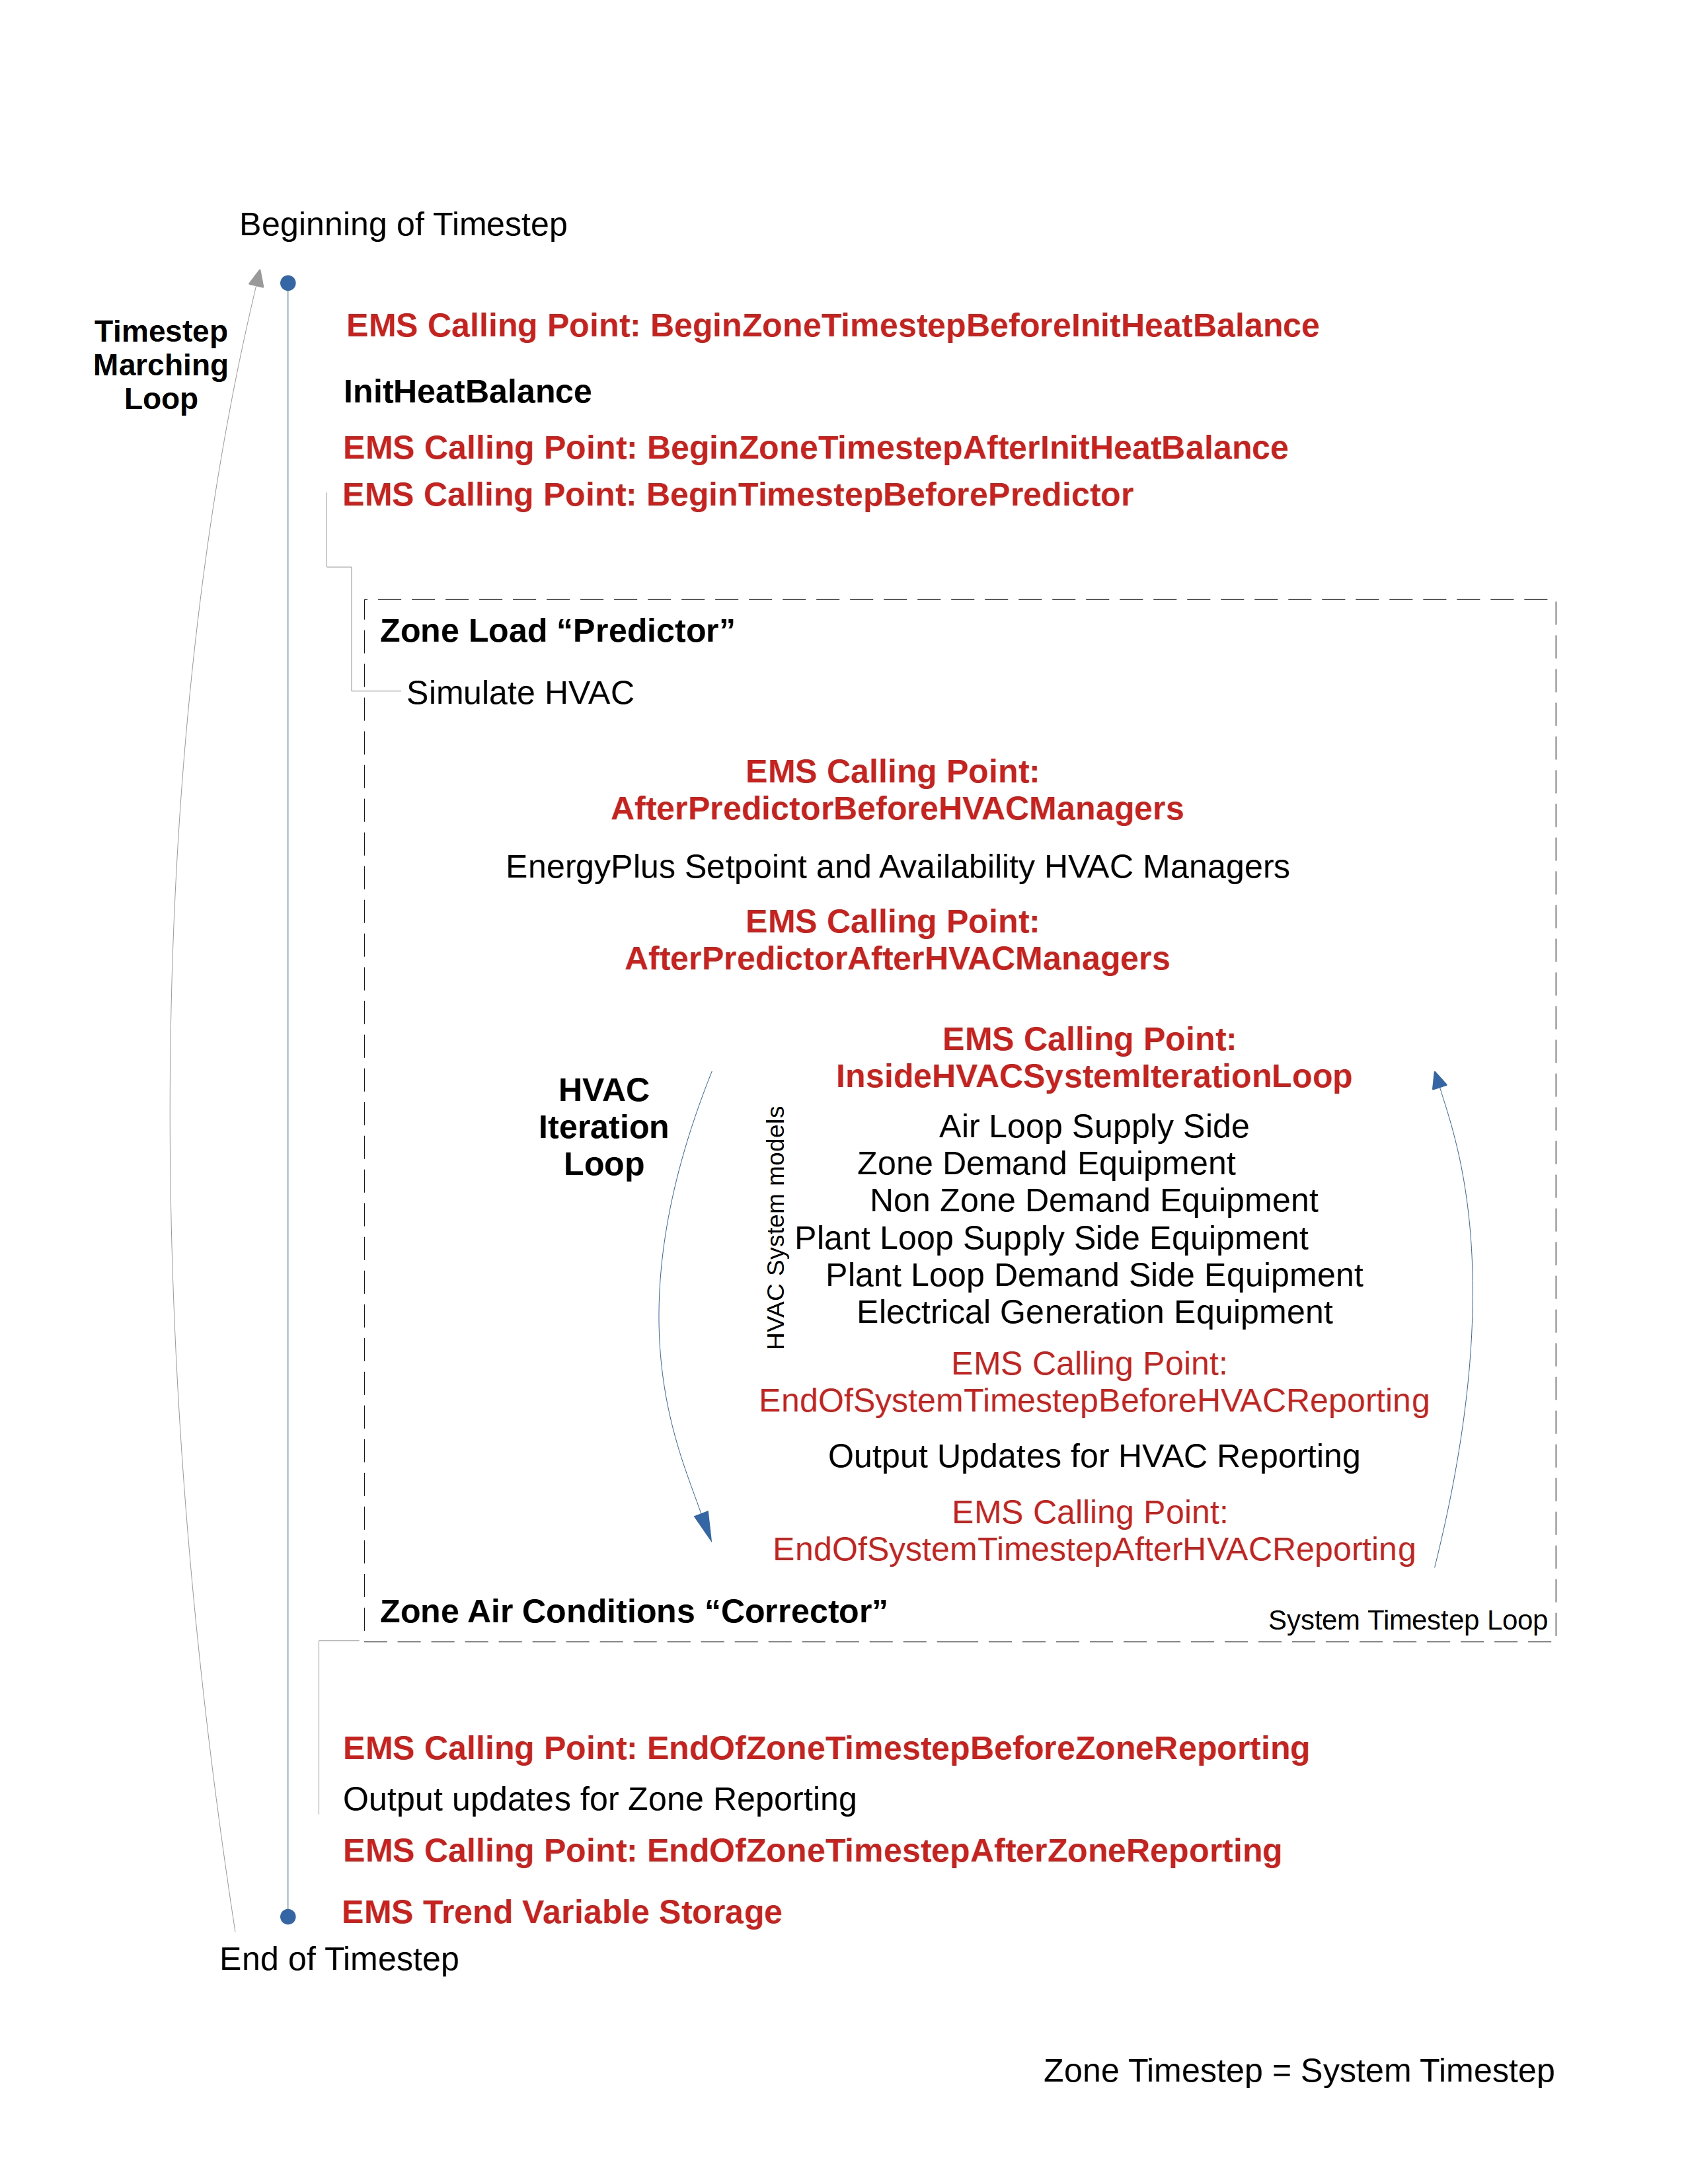
\includegraphics[width=0.9\textwidth, height=0.9\textheight, keepaspectratio=true]{media/image004.jpg}
\caption{Timestep Sequence with EMS Calling Points \protect \label{fig:timestep-sequence-with-ems-calling-points}}
\end{figure}

\begin{figure}[hbtp] % fig 3
\centering
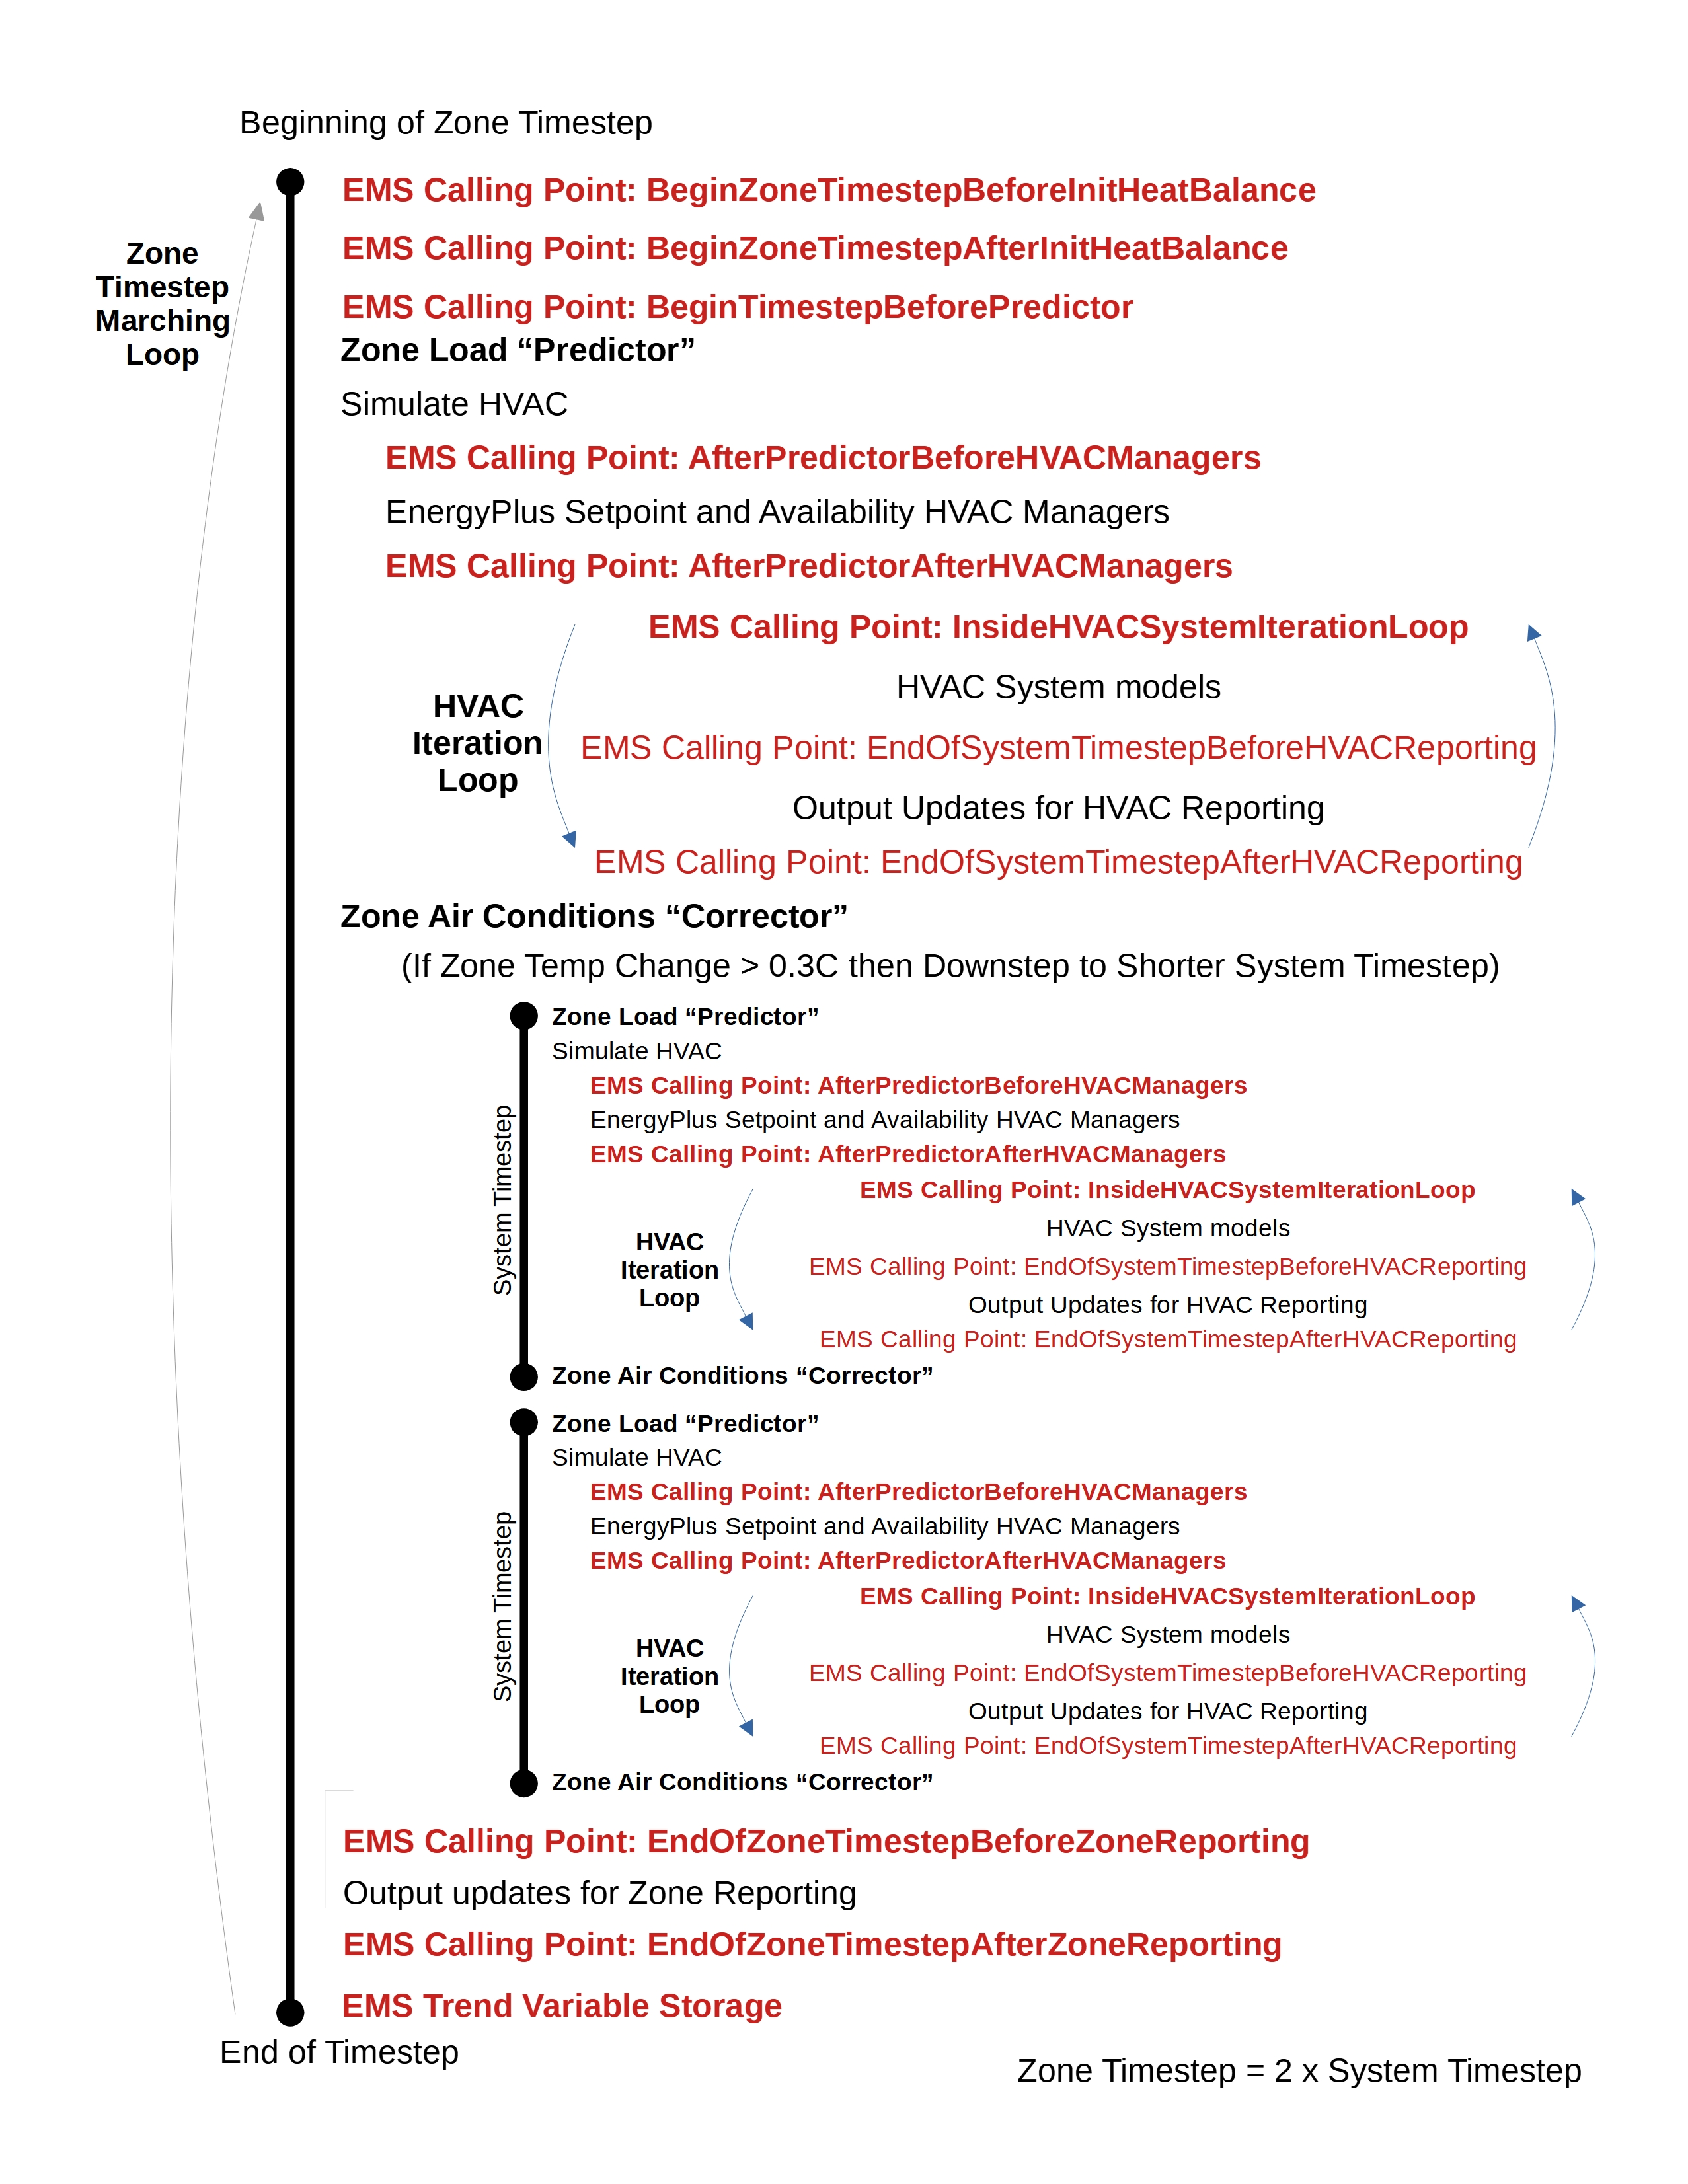
\includegraphics[width=0.9\textwidth, height=0.9\textheight, keepaspectratio=true]{media/image005.jpg}
\caption{System Timestep Sequence with EMS Calling Points \protect \label{fig:system-timestep-sequence-with-ems-calling}}
\end{figure}

When EnergyPlus runs a model, it first does various sizing and setup activities and then models the environment periods you ask for; e.g., design days and run periods. The built-in variable called CurrentEnvironment indentifies which of these is being simulated and any given time. Figure~\ref{fig:overall-program-flow-and-ems-calling-points} diagrams the overall program flow starting at the top and listing certain key steps in outline form. EnergyPlus models contain a lot of input, and the internal processes to acquire and process that input take some time to complete. Before the model starts doing final calculations, it may have to do various sizing calculations and automatically design the size of components. It will also go through special setup periods that model a truncated set of timesteps for each environment period. In the diagram, this initial phase is not finished until just before the design periods begin. Two EMS calling points that occur only once in a given run, EndOfZoneSizing and EndOfSystemSizing, can be triggered during this initial setup phase. During the phase called ``Setup Simulation,'' the various timestep-based calling points diagrammed in Figure~\ref{fig:timestep-sequence-with-ems-calling-points} will also be called.

Another thing that happens during the setup phase described above is that individual HVAC component models access their input data and do various setup calculations in preparation for the rest of the simulation.~~ An EMS calling point (added for Version 7) called ``AfterComponentInputReadIn'' is available for selected HVAC components that allows triggering Erl programs at a point just after the component's input data have been read in but before the component's sizing routines have executed.~ This calling point is intended to be used with various actuators that are setup to override the autosize values that result from sizing.

To model environment periods, EnergyPlus runs through a serious of timesteps. Figure~\ref{fig:timestep-sequence-with-ems-calling-points} diagrams the program flow for a single timestep where the timestep for the system modeling is equal to that for the zone load modeling. The \emph{system} timestep can be shorter than the \emph{zone} timestep. The usual process of modeling a timestep is to first calculate the zone loads during the ``Predictor,'' then model the response of the HVAC systems, and then calculate the resulting zone conditions during the ``Corrector.''~ Within the HVAC system modeling, some system iterations are used to iteratively solve a system of systems. Figure~\ref{fig:system-timestep-sequence-with-ems-calling} is a slightly modified version Figure~\ref{fig:timestep-sequence-with-ems-calling-points} that diagrams the situation when the timestep of the system calculations has been reduced to half the length of the zone timestep.
